\chapter{Configurazione dell'Ambiente di Sviluppo in Simulink per il Sistema PX4 Hardware-in-the-Loop (HITL)}
Per configurare il firmware PX4 per la simulazione Hardware-in-the-Loop (HITL), è necessario seguire i seguenti passaggi

\section{Configurazione QGroundControl}

Nella schermata di download di QGroundControl per la configurazione hardware, scarica e installa QGC.
Dopo l'installazione, clicca su "Verify Installation" per verificare che l'installazione sia avvenuta correttamente.
Successivamente, clicca su "Next" per procedere.
\\
Seguire questi passaggi per configurare e impostare QGroundControl (QGC):
\begin{itemize}
    \item Collegare l'autopilot a QGC tramite USB.
    \item Abilitare la modalità HITL.
    \item Navigare fino alla sezione Setup > Safety.
    \item Selezionare Enabled dalla lista HITL Enabled.
    \item Selezionare il telaio (Airframe).
    \item Navigare fino a Setup > Airframes.
    \item Selezionare HIL QuadCopter per simulare un quadricottero. Fare clic su Apply and Restart nella parte superiore destra della pagina di configurazione del telaio.
    \item Nella scheda Generale del menu delle impostazioni, deselezionare tutte le opzioni di AutoConnect tranne UDP.
    \\
    \textbf{Nota}: Questa selezione interrompe la comunicazione tra QGC e l'autopilot PX4 tramite USB. QGC può ora comunicare solo tramite UDP (di solito gestito da un Simulatore che funge da ponte tra QGC e l'autopilot e collega i dati MAVLink tra QGC e l'autopilota tramite UDP).
    \\
    \item Chiudere QGC.
\end{itemize}
\noindent

Continua con i passaggi successivi nel processo di configurazione hardware per la costruzione del firmware. 
\\
Assicurati di verificare che la compilazione sia avvenuta con successo.

\section{Configurazione del Modello del Controller PX4 in Simulink}
Eseguire questi passaggi per configurare il modello Simulink.

Nella scheda Modeling, fare clic su Model Settings.

Nella finestra di dialogo Configuration Parameters, selezionare PX4 Pixhawk 6x (Fig. \ref{fig:Hardware Board}).
\begin{figure}[H] % Opzione [h] posiziona la figura qui (here)
  \centering
  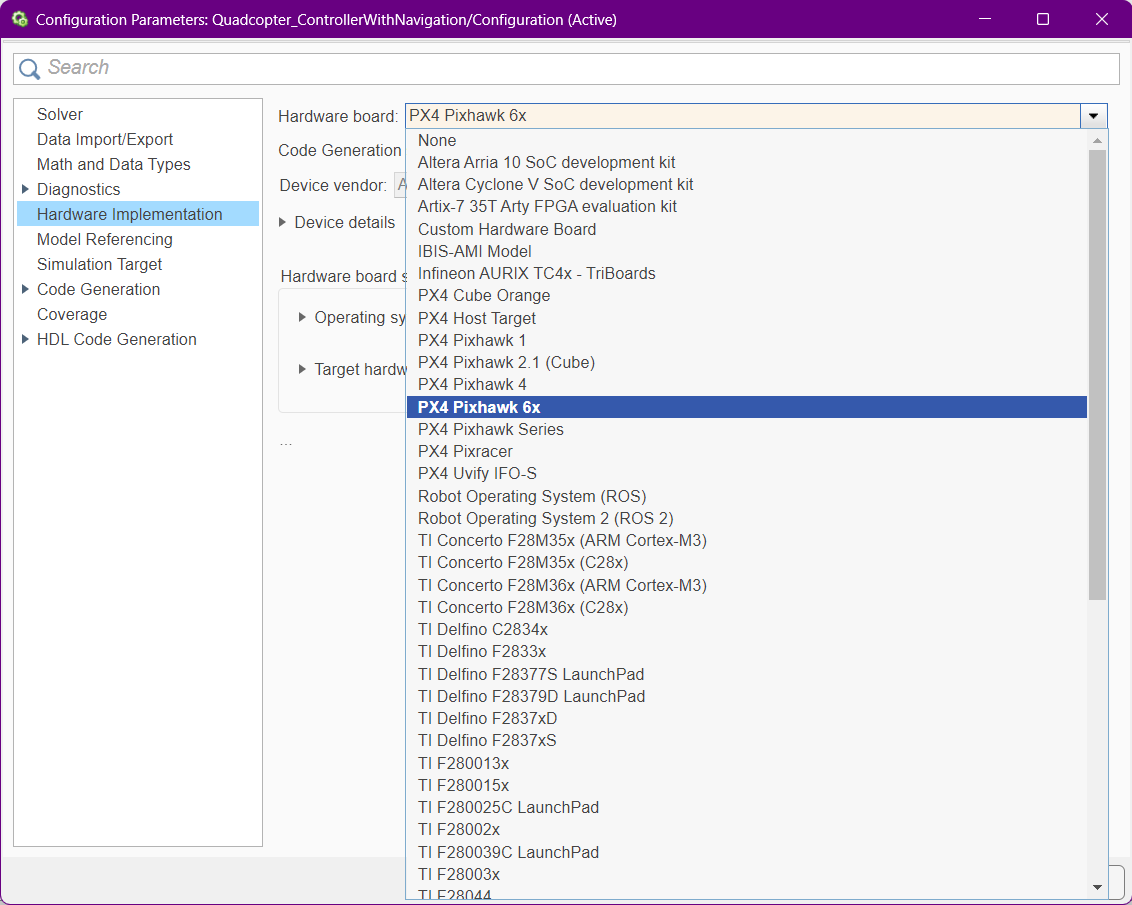
\includegraphics[width=0.8\textwidth]{files/images/matlab1.png} % Imposta la larghezza dell'immagine al 50% della larghezza del testo
  \caption{Hardware Board} % Didascalia sotto l'immagine
  \label{fig:Hardware Board} % Etichetta per fare riferimento all'immagine nel testo
\end{figure}
\noindent
Fare clic su HITL e quindi selezionare Enable HITL Mode (Fig. \ref{fig:HITL}).
\begin{figure}[H] % Opzione [h] posiziona la figura qui (here)
  \centering
  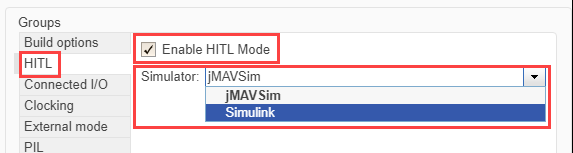
\includegraphics[width=0.8\textwidth]{files/images/HITL.png} % Imposta la larghezza dell'immagine al 50% della larghezza del testo
  \caption{HITL} % Didascalia sotto l'immagine
  \label{fig:HITL} % Etichetta per fare riferimento all'immagine nel testo
\end{figure}
\noindent
Selezionare il simulatore da eseguire per HITL.
\\
Fare clic su MAVLink e assicurarsi che l'opzione Enable MAVLink su /dev/ttyACM0 sia selezionata (Fig. \ref{fig:MAVLink}).
\begin{figure}[H] % Opzione [h] posiziona la figura qui (here)
  \centering
  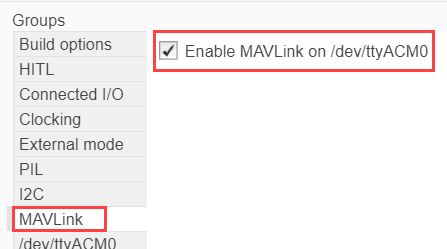
\includegraphics[width=0.8\textwidth]{files/images/MAVLink.png} % Imposta la larghezza dell'immagine al 50% della larghezza del testo
  \caption{MAVLink} % Didascalia sotto l'immagine
  \label{fig:MAVLink} % Etichetta per fare riferimento all'immagine nel testo
\end{figure}
\noindent
Fare clic su Apply e quindi su OK.


\section{Configurazione del Toolchain Cygwin e Download del Codice Sorgente PX4}
Questa sezione spiega il compito da completare come parte del passo "Configurazione del Toolchain Cygwin e Download del Codice Sorgente" del processo di configurazione hardware (utilizzando le schermate di configurazione hardware). 
\\
\textbf{Nota}: Assicurati che il tuo PC sia connesso a una connessione internet attiva prima di procedere con questo passaggio.
Per configurare il toolchain Cygwin™ e scaricare il codice sorgente PX4® utilizzato nel pacchetto di supporto per PX4 Autopilots nel UAV Toolbox, seguire questi passaggi:
\\
Scaricare la versione 0.8 di PX4 Cygwin Toolchain MSI Installer (Fig. \ref{fig:Download PX4 Cygwin Toolchain MSI Installer}), che è compatibile con PX4 Firmware v1.12.3, disponibile a questo \href{https://github.com/PX4/PX4-windows-toolchain/releases/tag/v0.8}{\textcolor{blue}{link}}.

\begin{figure}[H] % Opzione [h] posiziona la figura qui (here)
  \centering
  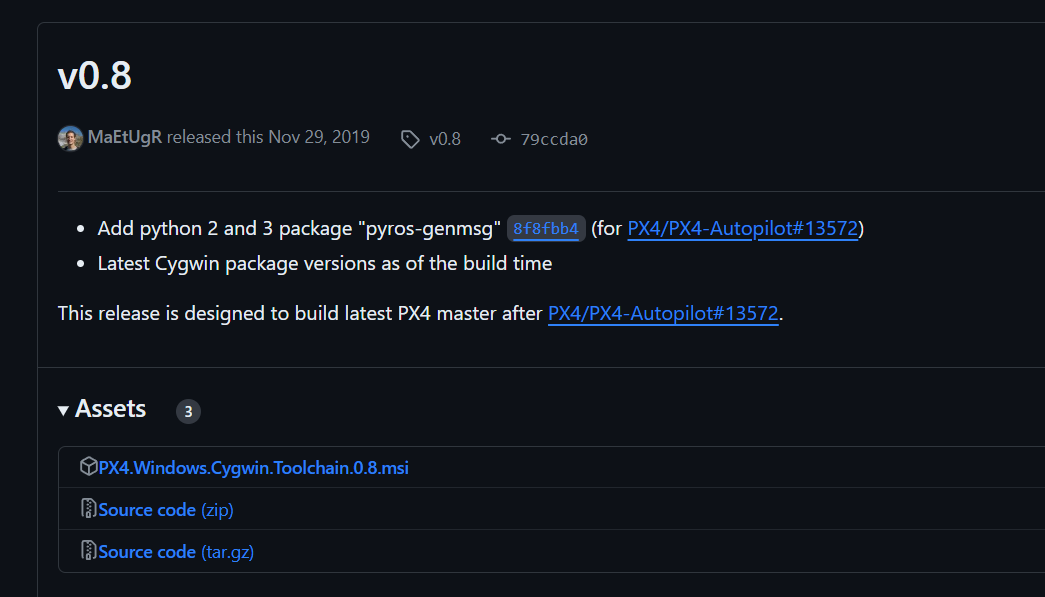
\includegraphics[width=0.8\textwidth]{files/images/github_cywing.png} % Imposta la larghezza dell'immagine al 50% della larghezza del testo
  \caption{Download PX4 Cygwin Toolchain MSI Installer} % Didascalia sotto l'immagine
  \label{fig:Download PX4 Cygwin Toolchain MSI Installer} % Etichetta per fare riferimento all'immagine nel testo
\end{figure}
\noindent
Nota: Il pacchetto di supporto UAV Toolbox per PX4 Autopilots supporta solo la versione v0.8 di PX4 Windows® Cygwin Toolchain MSI Installer, anche se una versione più recente potrebbe essere disponibile.
\\
Eseguire il programma di installazione MSI e avviare l'installazione del toolchain (Fig. \ref{fig:PX4 Toolchain Setup}).
\begin{figure}[H] % Opzione [h] posiziona la figura qui (here)
  \centering
  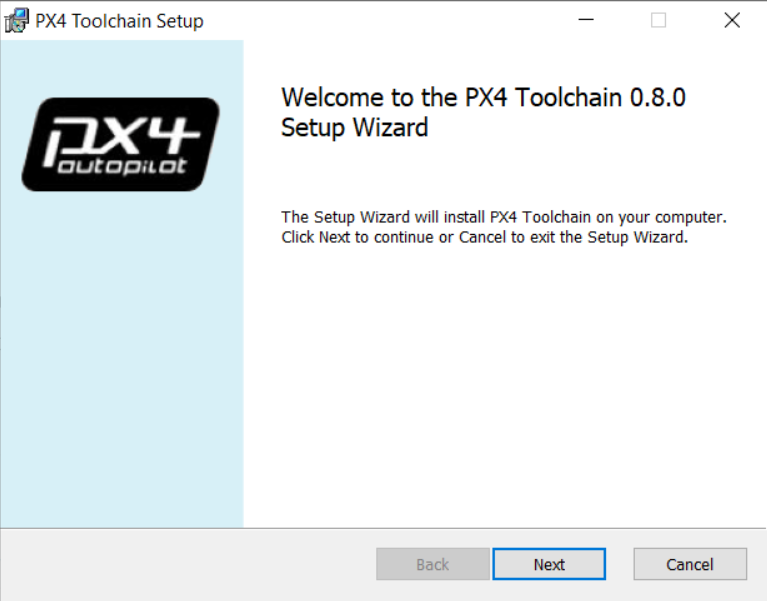
\includegraphics[width=0.8\textwidth]{files/images/setup_toolchain.png} % Imposta la larghezza dell'immagine al 50% della larghezza del testo
  \caption{PX4 Toolchain Setup} % Didascalia sotto l'immagine
  \label{fig:PX4 Toolchain Setup} % Etichetta per fare riferimento all'immagine nel testo
\end{figure}
\noindent
Cambiare la cartella di installazione per Cygwin in una qualsiasi cartella locale (ad esempio, C:\textbackslash{}px4), quindi fare clic su OK (Fig. \ref{fig:Selezione della cartella di installazione}).
\begin{figure}[H] % Opzione [h] posiziona la figura qui (here)
  \centering
  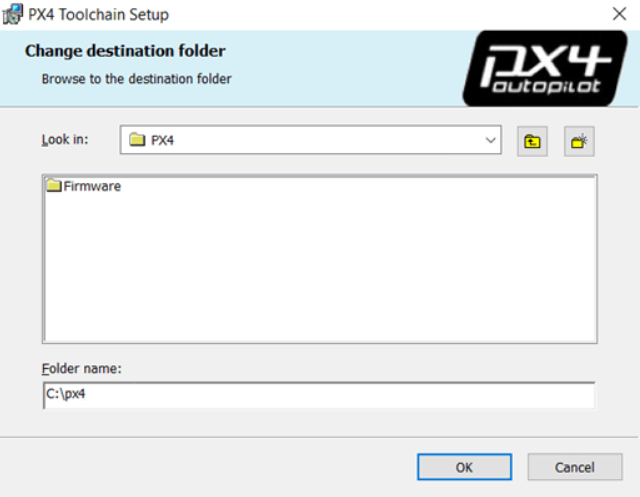
\includegraphics[width=0.8\textwidth]{files/images/folder_name.png} % Imposta la larghezza dell'immagine al 50% della larghezza del testo
  \caption{Selezione della cartella di installazione} % Didascalia sotto l'immagine
  \label{fig:Selezione della cartella di installazione} % Etichetta per fare riferimento all'immagine nel testo
\end{figure}
\noindent
All'ultimo passaggio della procedura guidata di configurazione del toolchain PX4, fare quanto segue:
\begin{itemize}
    \item Se non si dispone del Codice Sorgente PX4 (Firmware Autopilota PX4 v1.12.3) scaricato nel computer host, selezionare l'opzione "Clona repository PX4 e Avvia Simulazione", quindi fare clic su Fine. Questa opzione clona il firmware PX4 attuale. Quando si fa clic su Verifica Installazione nel passaggio 6 di seguito, il firmware viene automaticamente controllato alla versione v1.12.3.
    \item Se il Codice Sorgente PX4 (Firmware Autopilota PX4 v1.12.3) è già disponibile nel computer host, fare clic su Fine senza selezionare l'opzione "Clona repository PX4 e Avvia Simulazione" (Fig. \ref{fig:Clona repository PX4 e Avvia Simulazione}).
\end{itemize}
\begin{figure}[H] % Opzione [h] posiziona la figura qui (here)
  \centering
  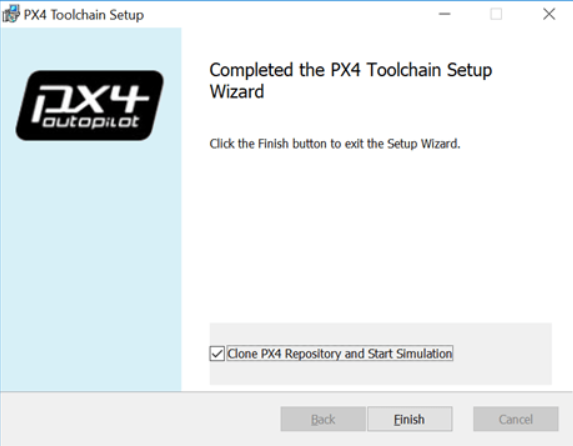
\includegraphics[width=0.8\textwidth]{files/images/clone_px4.png} % Imposta la larghezza dell'immagine al 50% della larghezza del testo
  \caption{Clona repository PX4 e Avvia Simulazione} % Didascalia sotto l'immagine
  \label{fig:Clona repository PX4 e Avvia Simulazione} % Etichetta per fare riferimento all'immagine nel testo
\end{figure}
\noindent
Se si è selezionata l'opzione "Clona repository PX4 e Avvia Simulazione" e si è fatto clic su Fine, viene avviata una shell bash che avvia la clonazione del firmware (Fig. \ref{fig:Shell bash che avvia la clonazione del firmware}).
\begin{figure}[H] % Opzione [h] posiziona la figura qui (here)
  \centering
  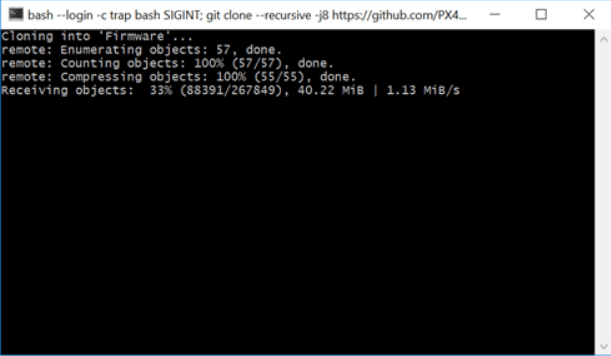
\includegraphics[width=0.8\textwidth]{files/images/bash_after_installation.png} % Imposta la larghezza dell'immagine al 50% della larghezza del testo
  \caption{Shell bash che avvia la clonazione del firmware} % Didascalia sotto l'immagine
  \label{fig:Shell bash che avvia la clonazione del firmware} % Etichetta per fare riferimento all'immagine nel testo
\end{figure}
\noindent
Attendere il completamento della clonazione del firmware. Dopo che il firmware è stato clonato, la Simulazione viene avviata in jMAVSim. È possibile chiudere la shell bash in questa fase.
\\
Il firmware PX4 viene clonato all'interno di una cartella denominata home, all'interno della cartella Cygwin selezionata durante l'installazione (ad esempio, C:\textbackslash{}px4\textbackslash{}home).

\section{Configurazione Firmware PX4 per l'Hardware-in-the-Loop}
Seguendo questi passaggi, il firmware PX4 sarà configurato correttamente per la simulazione Hardware-in-the-Loop (HITL) utilizzando il supporto per PX4 Autopilots nel UAV Toolbox. Questo ti permetterà di eseguire la simulazione HITL e verificare gli algoritmi di controllo implementati.
\\
Selezione del Firmware PX4 e del Hardware di Destinazione:
\\
Accedi alla schermata di selezione del firmware PX4 e del hardware di destinazione nel UAV Toolbox Support Package for PX4 Autopilots. Clicca su "Manage" (Fig. \ref{fig:UAV Toolbox Support Package for PX4 Autopilots}) e successivamente su "setup" (Fig. \ref{fig:Manage Toolbox}).

\begin{figure}[htbp]
    \begin{minipage}[b]{0.5\linewidth} % Definisci la larghezza della prima minipage (50% della larghezza della pagina)
        \centering
        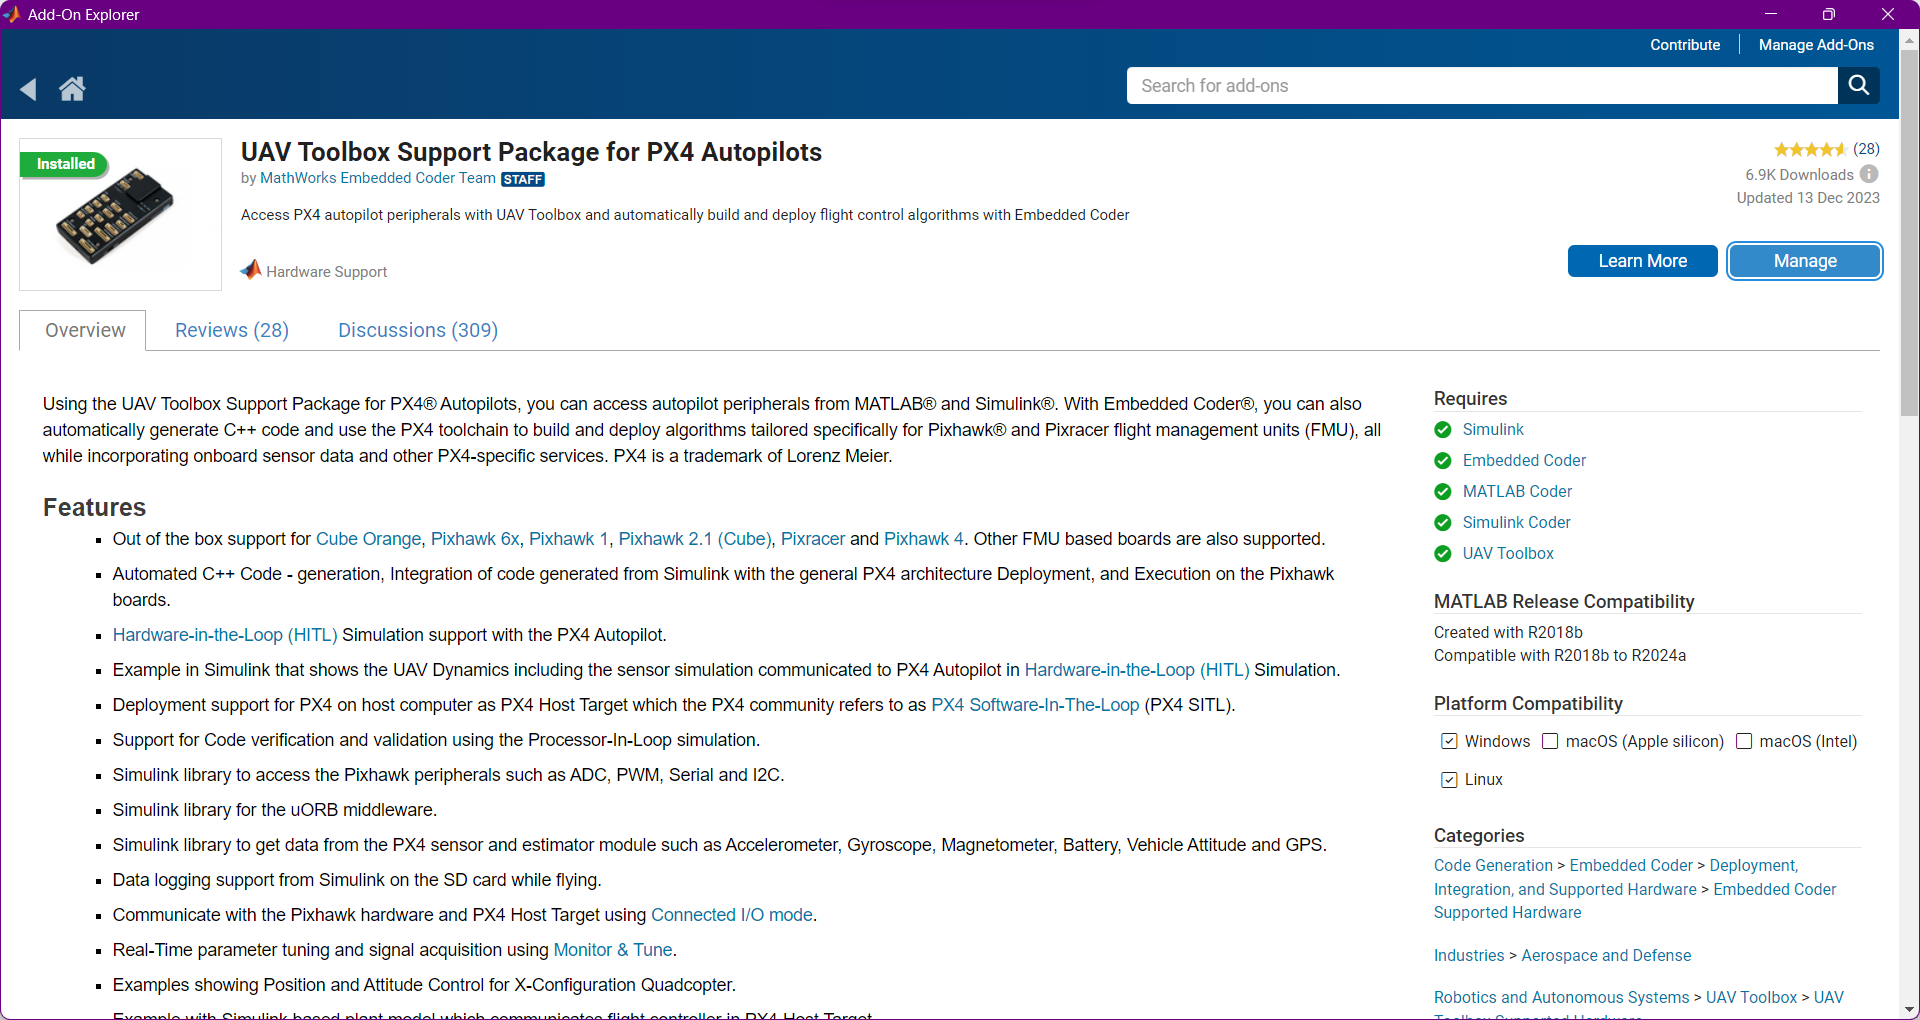
\includegraphics[width=\linewidth]{files/images/Screenshot 2024-03-13 120711.png} % Inserisci la prima immagine
        \caption{UAV Toolbox Support Package for PX4 Autopilots}
        \label{fig:UAV Toolbox Support Package for PX4 Autopilots}
    \end{minipage}%
    \begin{minipage}[b]{0.5\linewidth} % Definisci la larghezza della seconda minipage (50% della larghezza della pagina)
        \centering
        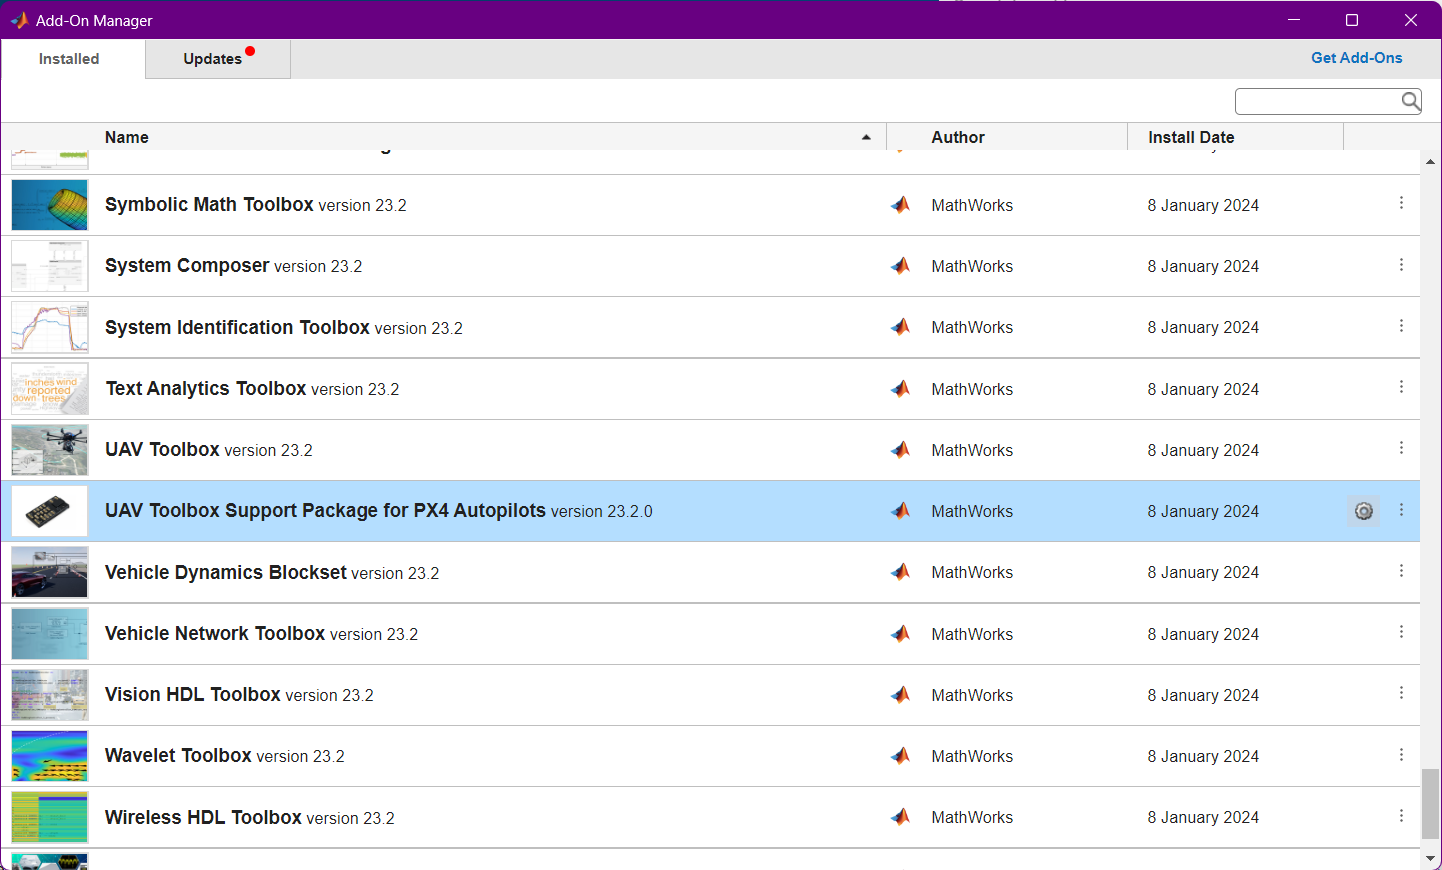
\includegraphics[width=\linewidth]{files/images/Screenshot 2024-03-13 120731.png} % Inserisci la seconda immagine
        \caption{Manage Toolbox}
        \label{fig:Manage Toolbox}
    \end{minipage}
\end{figure}

Una volta aperto l'Hardware Setup, inserire il percorso utilizzato per l'installazione del toolchain Cygwin (stesso percorso della Figura \ref{fig:Selezione della cartella di installazione}), quindi fare clic su Verifica Installazione (Fig. \ref{fig:Verifica Percorso}).
\begin{figure}[H] % Opzione [h] posiziona la figura qui (here)
  \centering
  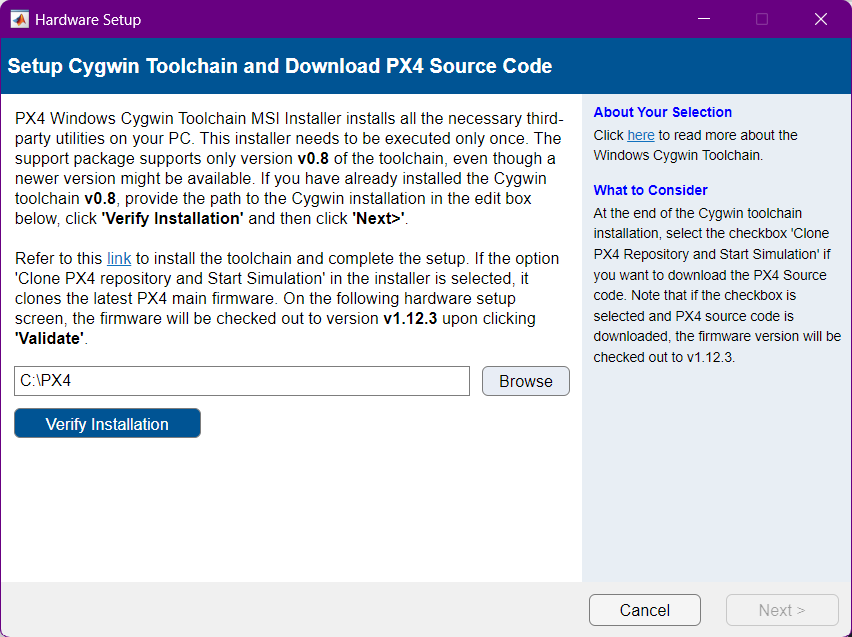
\includegraphics[width=0.7\textwidth]{files/images/matlab3.png} % Imposta la larghezza dell'immagine al 50% della larghezza del testo
  \caption{Verifica Percorso} % Didascalia sotto l'immagine
  \label{fig:Verifica Percorso} % Etichetta per fare riferimento all'immagine nel testo
\end{figure}
\noindent
Una volta uscita una spunta verde, clicca Next (Fig. \ref{fig:Verifica Percorso andata a buon fine}).
\begin{figure}[H] % Opzione [h] posiziona la figura qui (here)
  \centering
  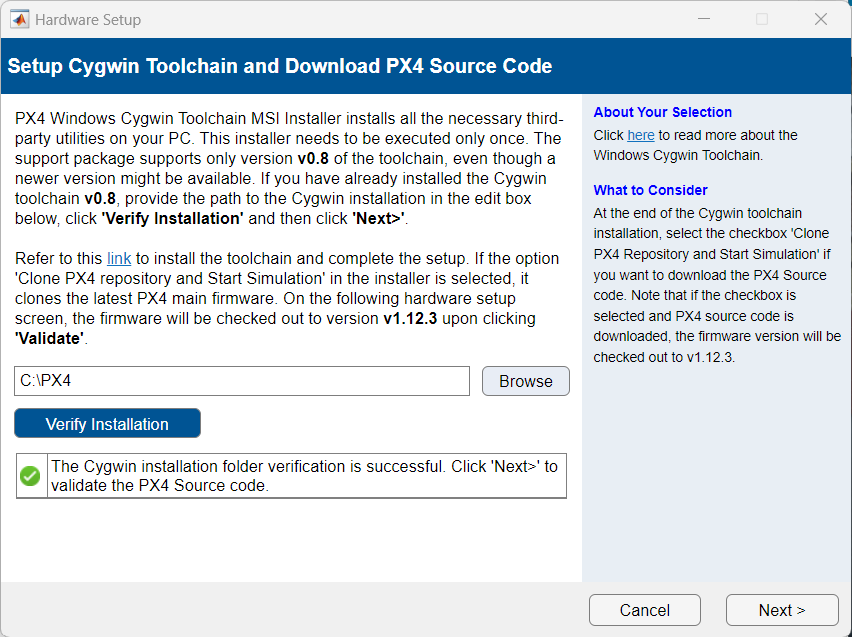
\includegraphics[width=0.7\textwidth]{files/images/matlab4.png} % Imposta la larghezza dell'immagine al 50% della larghezza del testo
  \caption{Verifica Percorso andata a buon fine} % Didascalia sotto l'immagine
  \label{fig:Verifica Percorso andata a buon fine} % Etichetta per fare riferimento all'immagine nel testo
\end{figure}
\noindent
Selezionare la cartella di download per il codice sorgente della PX4 (Fig. \ref{fig:Cartella di download per il codice sorgente della PX4}).
\begin{figure}[H] % Opzione [h] posiziona la figura qui (here)
  \centering
  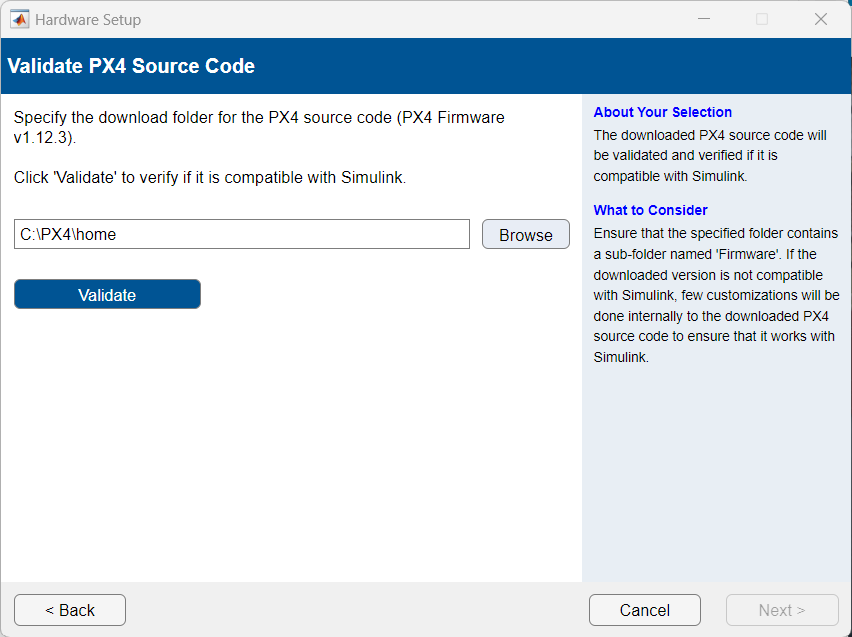
\includegraphics[width=0.7\textwidth]{files/images/matlab5.png} % Imposta la larghezza dell'immagine al 50% della larghezza del testo
  \caption{Cartella di download per il codice sorgente della PX4} % Didascalia sotto l'immagine
  \label{fig:Cartella di download per il codice sorgente della PX4} % Etichetta per fare riferimento all'immagine nel testo
\end{figure}
\noindent
Aspettare che esca la scritta "Firmware validation successful" e clicca "Next" (Fig. \ref{fig:Firmware validation successful}).
\begin{figure}[H] % Opzione [h] posiziona la figura qui (here)
  \centering
  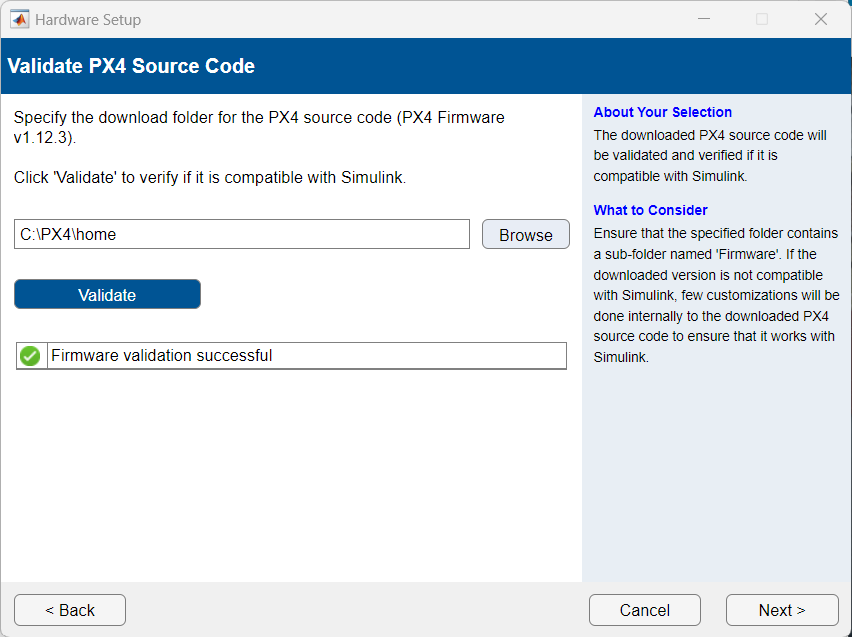
\includegraphics[width=0.7\textwidth]{files/images/matlab6.png} % Imposta la larghezza dell'immagine al 50% della larghezza del testo
  \caption{Firmware validation successful} % Didascalia sotto l'immagine
  \label{fig:Firmware validation successful} % Etichetta per fare riferimento all'immagine nel testo
\end{figure}
\noindent
Selezionare "Design Flight Controller in Simulink" e clicca "Next" (Fig. \ref{fig:Design Flight Controller in Simulink}) 
\begin{figure}[H] % Opzione [h] posiziona la figura qui (here)
  \centering
  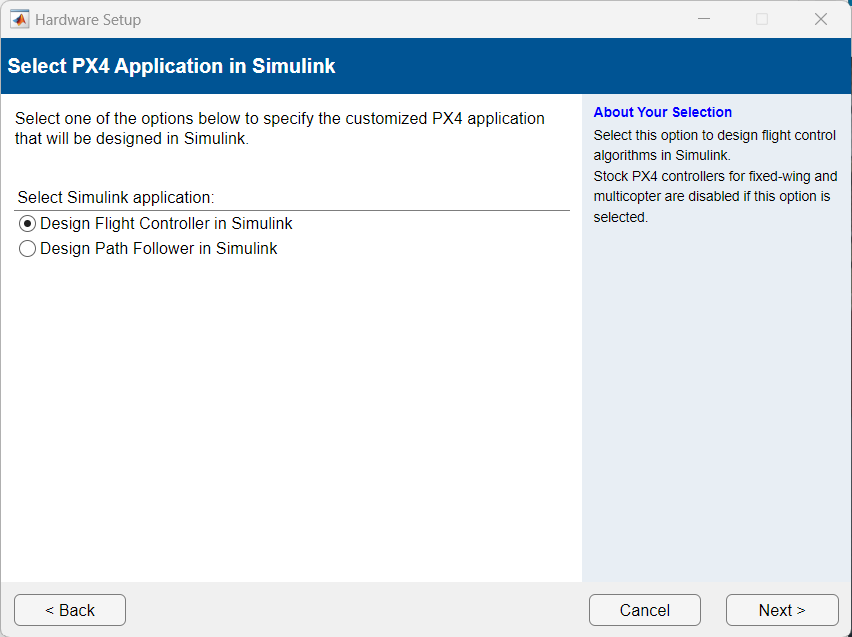
\includegraphics[width=0.7\textwidth]{files/images/matlab7.png} % Imposta la larghezza dell'immagine al 50% della larghezza del testo
  \caption{Design Flight Controller in Simulink} % Didascalia sotto l'immagine
  \label{fig:Design Flight Controller in Simulink} % Etichetta per fare riferimento all'immagine nel testo
\end{figure}
\noindent
Selezionare la "PX4 Pixhawk 6x" con build target "px4\_fmu\-v6x\_multicopter" e clicca "Next" (Fig. \ref{fig:Select a PX4 Autopilot and Build Target}).
\begin{figure}[H] % Opzione [h] posiziona la figura qui (here)
  \centering
  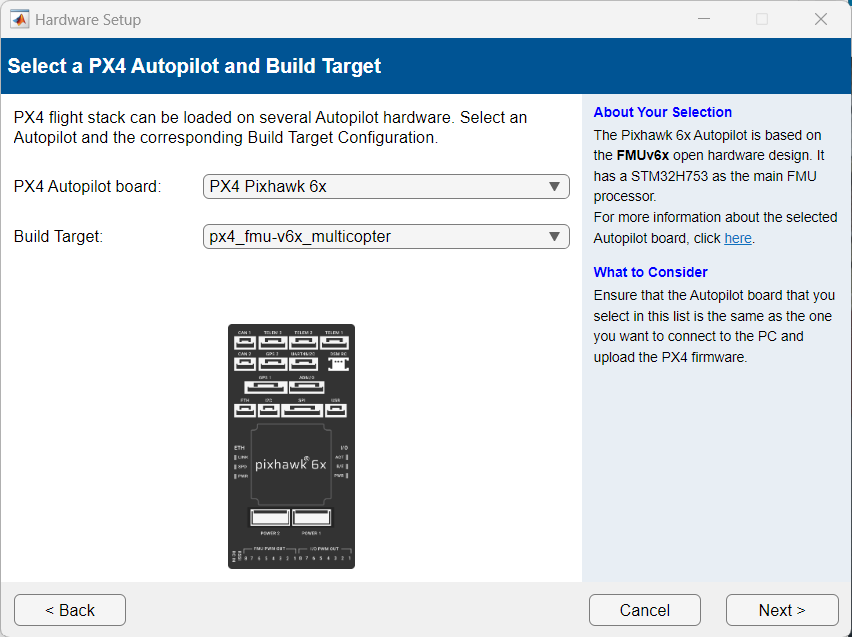
\includegraphics[width=0.7\textwidth]{files/images/matlab8.png} % Imposta la larghezza dell'immagine al 50% della larghezza del testo
  \caption{Select a PX4 Autopilot and Build Target} % Didascalia sotto l'immagine
  \label{fig:Select a PX4 Autopilot and Build Target} % Etichetta per fare riferimento all'immagine nel testo
\end{figure}
\noindent
Selezionare "Use default starup script" e clicca "Next" (Fig. \ref{fig:Select System Startup Script in PX4}).
\begin{figure}[H] % Opzione [h] posiziona la figura qui (here)
  \centering
  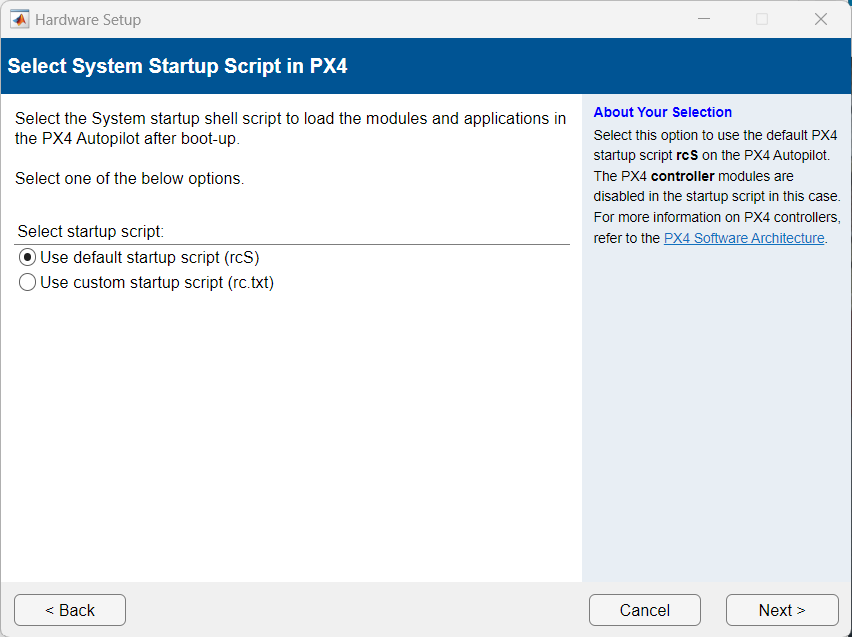
\includegraphics[width=0.7\textwidth]{files/images/matlab9.png} % Imposta la larghezza dell'immagine al 50% della larghezza del testo
  \caption{Select System Startup Script in PX4} % Didascalia sotto l'immagine
  \label{fig:Select System Startup Script in PX4} % Etichetta per fare riferimento all'immagine nel testo
\end{figure}
\noindent
Verificare la installazione di QGroundControl e cliccare "Next" (Fig. \ref{fig:Download QGroundControl} e Fig. \ref{fig:Download QGroundControl Successful}).
\begin{figure}[H] % Opzione [h] posiziona la figura qui (here)
  \centering
  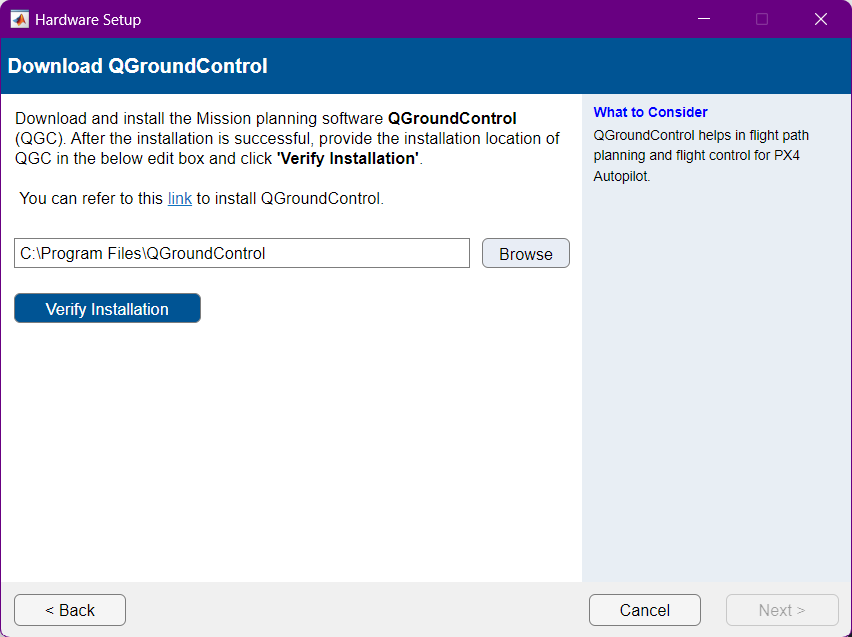
\includegraphics[width=0.7\textwidth]{files/images/matlab10.png} % Imposta la larghezza dell'immagine al 50% della larghezza del testo
  \caption{Download QGroundControl} % Didascalia sotto l'immagine
  \label{fig:Download QGroundControl} % Etichetta per fare riferimento all'immagine nel testo
\end{figure}
\noindent
\begin{figure}[H] % Opzione [h] posiziona la figura qui (here)
  \centering
  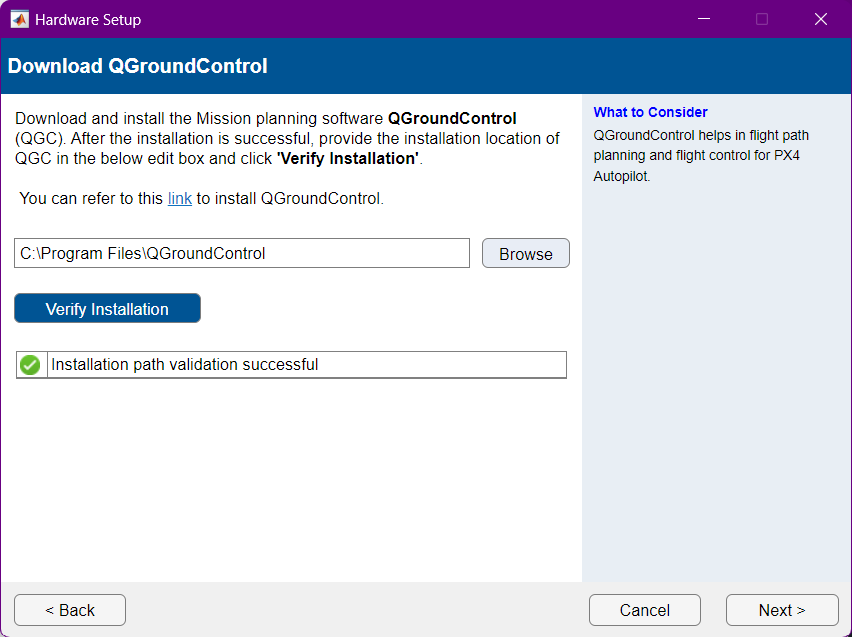
\includegraphics[width=0.7\textwidth]{files/images/matlab11.png} % Imposta la larghezza dell'immagine al 50% della larghezza del testo
  \caption{Download QGroundControl Successful} % Didascalia sotto l'immagine
  \label{fig:Download QGroundControl Successful} % Etichetta per fare riferimento all'immagine nel testo
\end{figure}
\noindent
Clicca "Next" (Fig. \ref{fig:Select Airframe in QGroundControl}).
\begin{figure}[H] % Opzione [h] posiziona la figura qui (here)
  \centering
  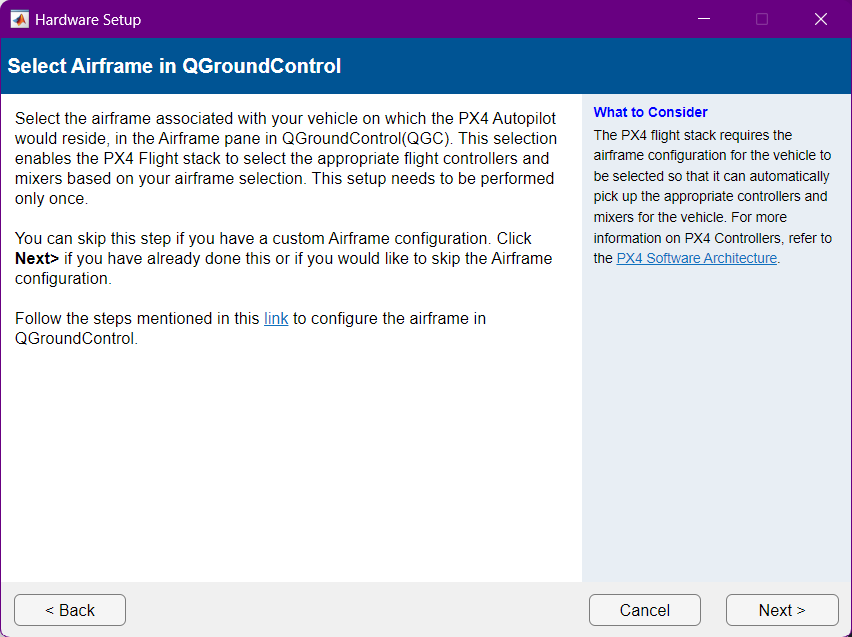
\includegraphics[width=0.7\textwidth]{files/images/matlab12.png} % Imposta la larghezza dell'immagine al 50% della larghezza del testo
  \caption{Select Airframe in QGroundControl} % Didascalia sotto l'immagine
  \label{fig:Select Airframe in QGroundControl} % Etichetta per fare riferimento all'immagine nel testo
\end{figure}
\noindent
Spuntere la casella "Delete PX4 Build folder for all CMake Configurations before building Firmware" ed eseguire il Build del Firmware (Fig. \ref{fig:Build Firmware}).
\begin{figure}[H] % Opzione [h] posiziona la figura qui (here)
  \centering
  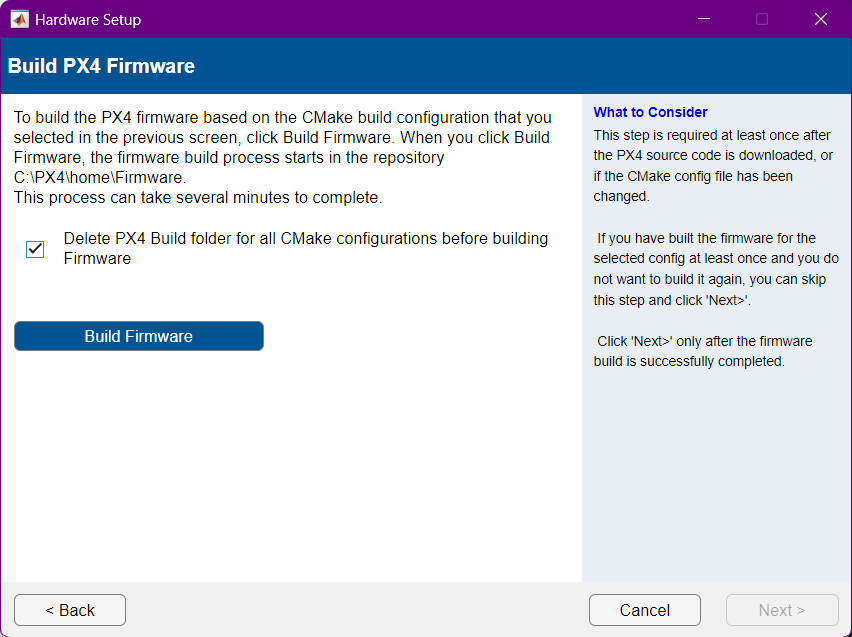
\includegraphics[width=0.7\textwidth]{files/images/matlab13.png} % Imposta la larghezza dell'immagine al 50% della larghezza del testo
  \caption{Build Firmware} % Didascalia sotto l'immagine
  \label{fig:Build Firmware} % Etichetta per fare riferimento all'immagine nel testo
\end{figure}
\noindent
Aspettare finchè non esce la scritta "Firmware Build Successful" e clicca "Next" (Fig. \ref{fig:Firmware Building} e Fig. \ref{fig:Firmware build successful}).
\begin{figure}[htbp]
    \begin{minipage}[b]{0.5\linewidth} % Definisci la larghezza della prima minipage (50% della larghezza della pagina)
      \centering
      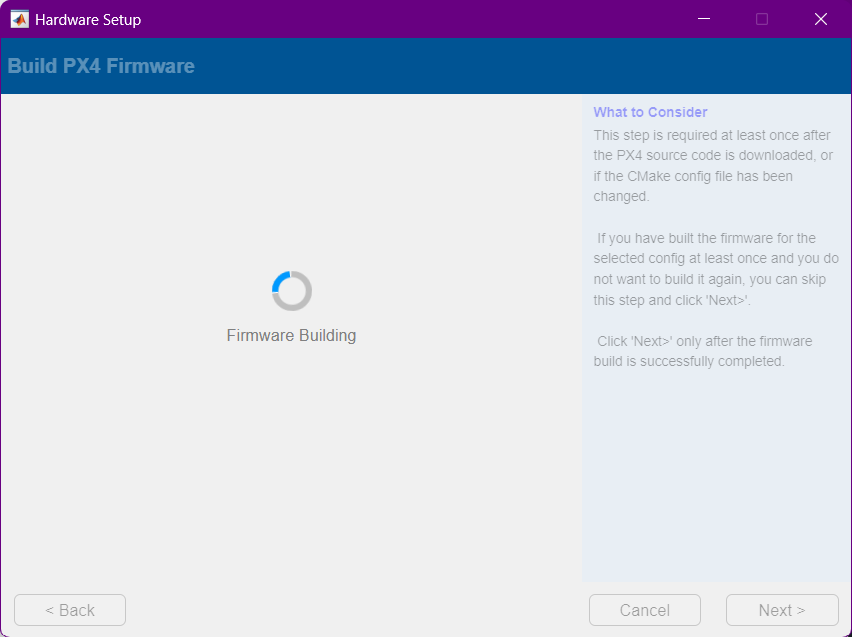
\includegraphics[width=\linewidth]{files/images/matlab14.png} % Imposta la larghezza dell'immagine al 50% della larghezza del testo
      \caption{Firmware Building} % Didascalia sotto l'immagine
      \label{fig:Firmware Building} % Etichetta per fare riferimento all'immagine nel testo
    \end{minipage}%
    \begin{minipage}[b]{0.5\linewidth} % Definisci la larghezza della seconda minipage (50% della larghezza della pagina)
        \centering
        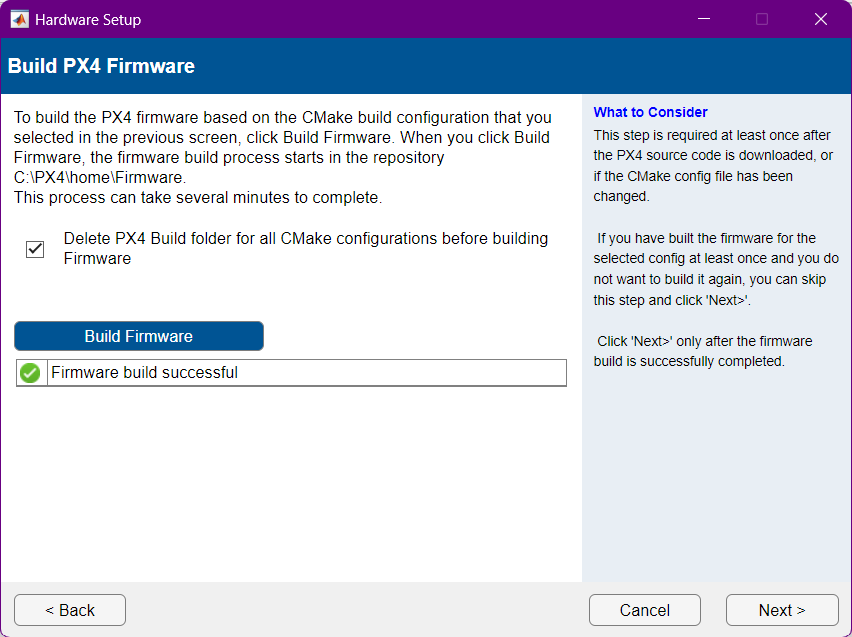
\includegraphics[width=\linewidth]{files/images/matlab15.png} % Imposta la larghezza dell'immagine al 50% della larghezza del testo
        \caption{Firmware build successful} % Didascalia sotto l'immagine
      \label{fig:Firmware build successful} % Etichetta per fare riferimento all'immagine nel
    \end{minipage}
\end{figure}
\noindent
Selezionare la COM a cui è collegata la PX4 ed eseguire il caricamento del firmware (Fig. \ref{fig:Test Connection}).
\begin{figure}[H] % Opzione [h] posiziona la figura qui (here)
  \centering
  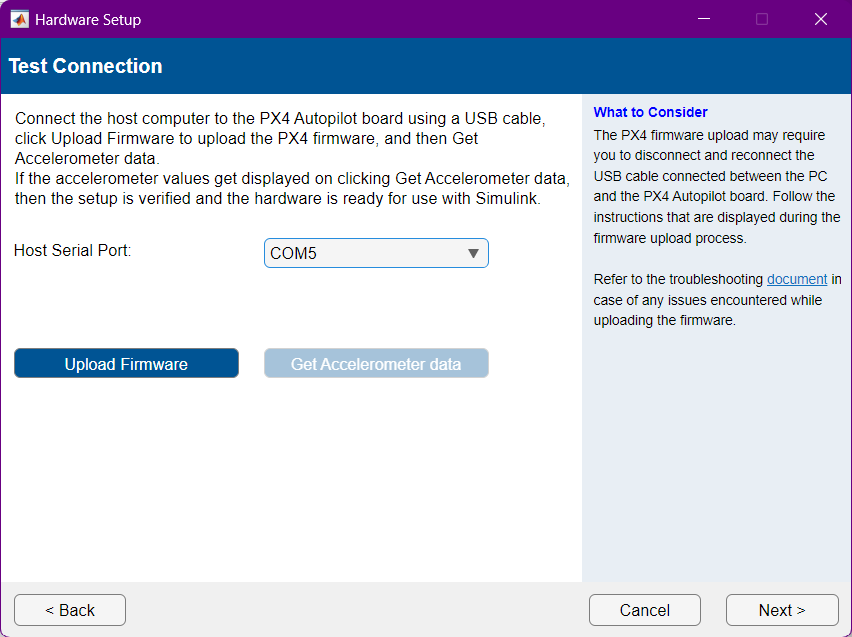
\includegraphics[width=0.7\textwidth]{files/images/matlab16.png} % Imposta la larghezza dell'immagine al 50% della larghezza del testo
  \caption{Test Connection} % Didascalia sotto l'immagine
  \label{fig:Test Connection} % Etichetta per fare riferimento all'immagine nel testo
\end{figure}
\noindent
Uscirà il messaggio mostrato in figura \ref{fig:Reconnect Pixhawk 6x}, clicca "OK" e scollegare la PX4 dal pc. Quindi togliere il cavo USB c e collegarlo nuovamente per il riavvio della PX4.
\begin{figure}[H] % Opzione [h] posiziona la figura qui (here)
  \centering
  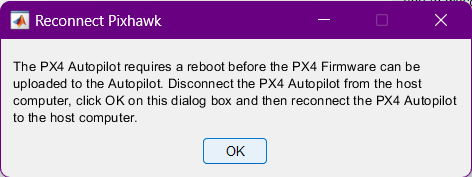
\includegraphics[width=0.7\textwidth]{files/images/matlab17.png} % Imposta la larghezza dell'immagine al 50% della larghezza del testo
  \caption{Reconnect Pixhawk 6x} % Didascalia sotto l'immagine
  \label{fig:Reconnect Pixhawk 6x} % Etichetta per fare riferimento all'immagine nel testo
\end{figure}
\noindent
A questo punto verrà effettuato il caricamento del firmware nella PX4, quindi aspettare il suo completamento (Fig. \ref{fig:Firmware uploading} e Fig. \ref{fig:Firmware upload successful}).


\begin{figure}[htbp]
    \begin{minipage}[b]{0.5\linewidth} % Definisci la larghezza della prima minipage (50% della larghezza della pagina)
      \centering
      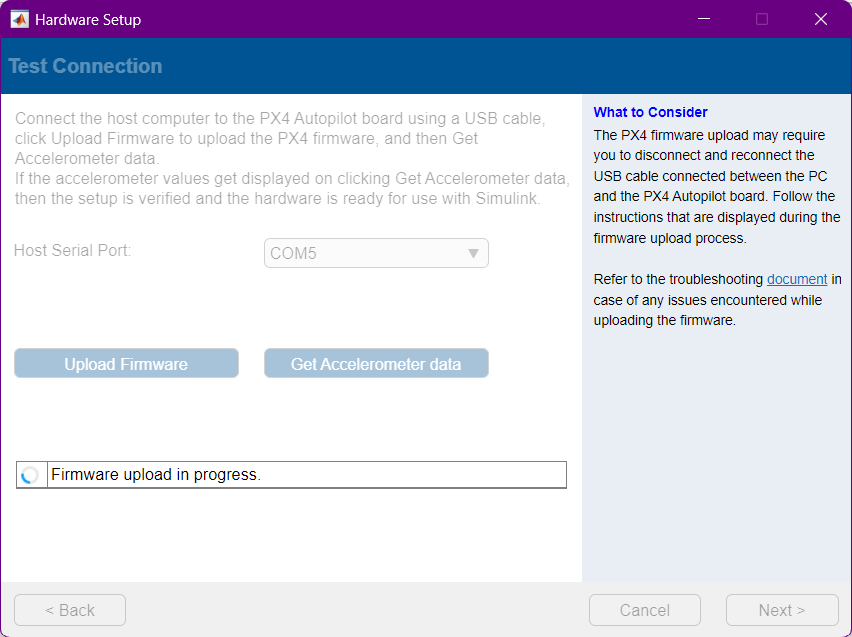
\includegraphics[width=\linewidth]{files/images/matlab18.png} % Imposta la larghezza dell'immagine al 50% della larghezza del testo
      \caption{Firmware uploading} % Didascalia sotto l'immagine
      \label{fig:Firmware uploading} % Etichetta per fare riferimento all'immagine nel testo
    \end{minipage}%
    \begin{minipage}[b]{0.5\linewidth} % Definisci la larghezza della seconda minipage (50% della larghezza della pagina)
        \centering
        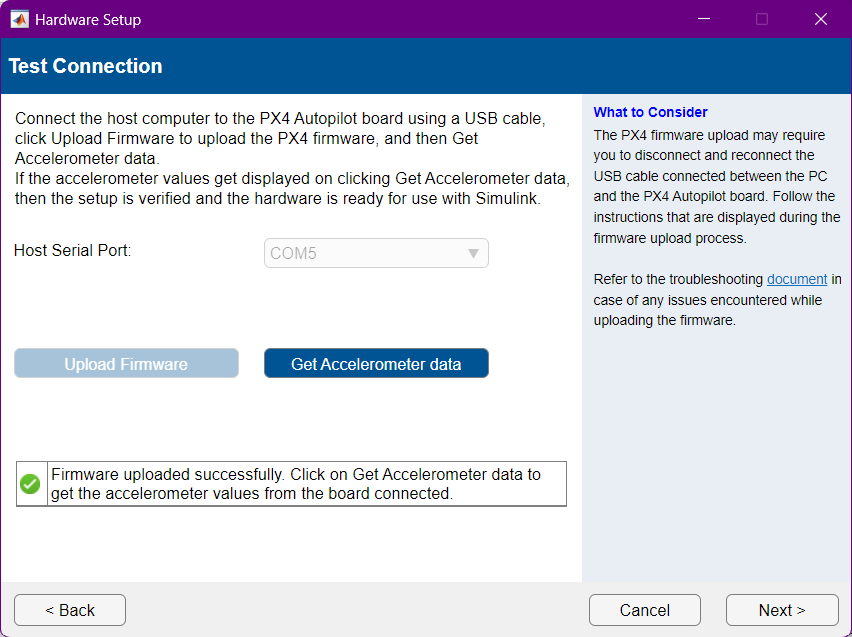
\includegraphics[width=\linewidth]{files/images/matlab19.png} % Imposta la larghezza dell'immagine al 50% della larghezza del testo
        \caption{Firmware upload successful} % Didascalia sotto l'immagine
      \label{fig:Firmware upload successful} % Etichetta per fare riferimento all'immagine nel
    \end{minipage}
\end{figure}
\noindent
A questo punto è terminata la configurazione del firmware per la PX4.

\section{Avvio Simulazione}
\subsection{Collegamento Hardware}
Come primo passo si collega la Pixhawk al computer host usando il cavo USB c, successivamente si collega la porta seriale a telem3 (/dev/ttyS7) e la porta USB sul computer host utilizzando un convertitore Serial-to-USB FTDI come mostrato nell'immagine di esempio qui sotto (Fig. \ref{fig:Collegamento PX4 Pixhawk 6x}).
\begin{figure}[H] % Opzione [h] posiziona la figura qui (here)
  \centering
  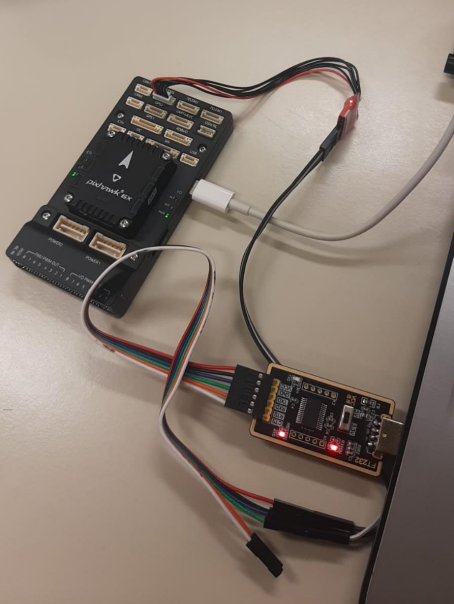
\includegraphics[width=0.5\textwidth]{files/images/collegamento_px4.png} % Imposta la larghezza dell'immagine al 50% della larghezza del testo
  \caption{Collegamento PX4 Pixhawk 6x} % Didascalia sotto l'immagine
  \label{fig:Collegamento PX4 Pixhawk 6x} % Etichetta per fare riferimento all'immagine nel testo
\end{figure}
\noindent


\subsection{Configurare il Modello}
 Una volta collegata la PX4, si va a configurare il modello Simulink e l'abilitazione per la calibrazione dei parametri negli strumenti di calibrazione di terze parti.
\\
Nota: Questi passaggi non sono necessari nel modello preconfigurato. Eseguire questi passaggi se hai modificato l'hardware o non stai utilizzando il modello preconfigurato.
\\
\begin{itemize}
    \item Apri il modello.
    \item Vai su Modeling > Model Settings per aprire la finestra di dialogo Configuration Parameters.
    \item Apri il pannello Hardware Implementation e seleziona la scheda PX4 Pixhawk 6x.
    \item Espandi le risorse hardware di destinazione per quella scheda.
    \item Fai clic su HITL e quindi seleziona Enable HITL Mode. Abilitando la modalità HITL, il simulatore jMAVSim e QGC vengono automaticamente configurati e avviati per essere eseguiti insieme al modello Simulink.
    \item Fai clic su External mode e seleziona /dev/ttyS7 come porta seriale della scheda hardware. Nel parametro Host Serial port, inserisci il numero di porta seriale host sul computer host per la comunicazione in modalità esterna.
    \item Fai clic su MAVLink e assicurati che sia selezionata l'opzione Enable MAVLink on /dev/ttyACM0.
    \item Fai clic su /dev/ttyS7 e imposta il Baud rate su 921600. Non modificare altri parametri.
    \item Fai clic su Apply e poi su OK.
\end{itemize}

\subsection{Avviare Monitor e Azione di Sintonizzazione per il Modello}
\begin{itemize}
    \item Nella scheda Hardware, nella sezione Mode, seleziona Run on board e poi fai clic su Monitor \& Tune.
    \item Questo avvia QGC
    \item In QGC, vai alla vista Plan.
    \item Crea una missione o carica la missione pre-pianificata, Mission.plan, disponibile con questo in figura \ref{fig:Test Volo with Unreal Enginee}.
    \begin{figure}[H] % Opzione [h] posiziona la figura qui (here)
      \centering
      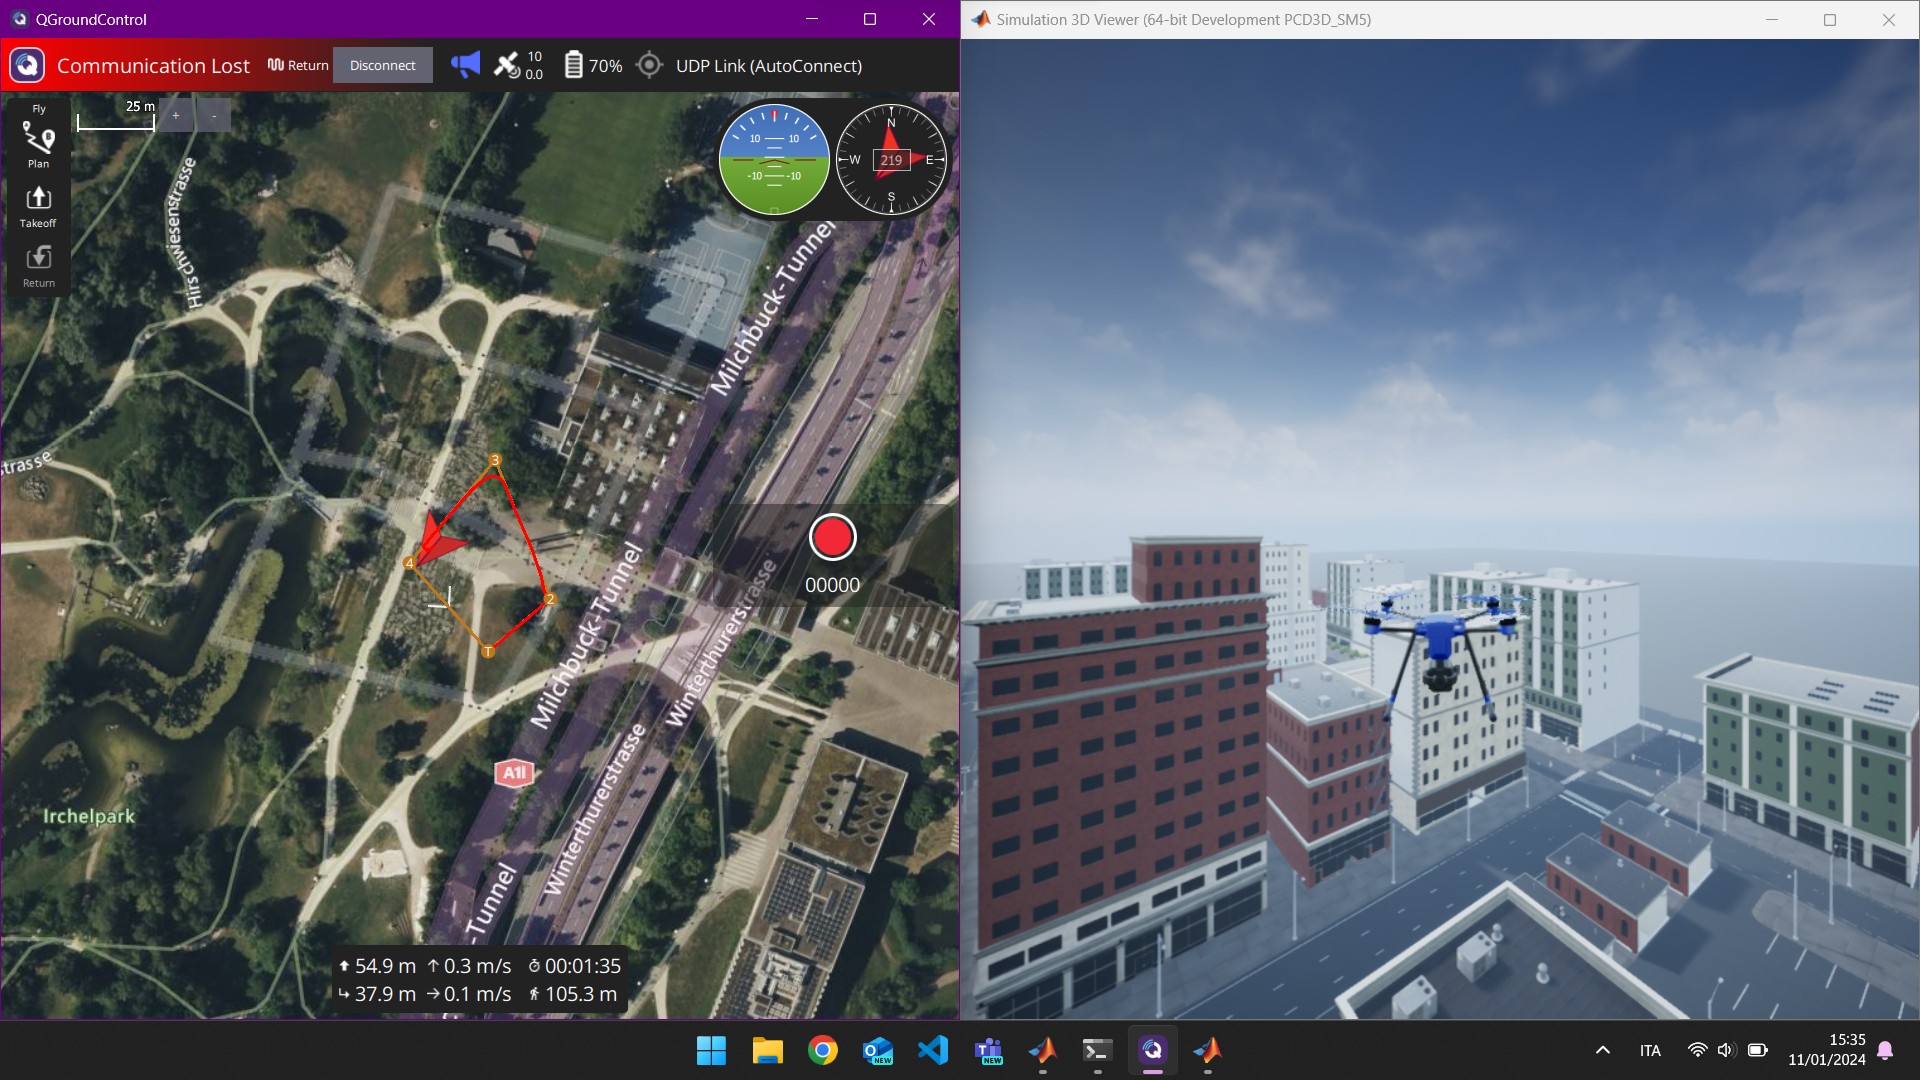
\includegraphics[width=0.8\textwidth]{files/images/test_volo.png} % Imposta la larghezza dell'immagine al 50% della larghezza del testo
      \caption{Test Volo with Unreal Enginee} % Didascalia sotto l'immagine
      \label{fig:Test Volo with Unreal Enginee} % Etichetta per fare riferimento all'immagine nel testo
    \end{figure}
\noindent
    \item Crea una missione: Per informazioni su come creare una missione, consulta Plan View.
    \item Carica una missione: Fai clic su Open Example nella parte superiore di questa pagina per salvare il file di piano sul tuo computer. Dopo aver salvato il file .plan, avvia QGC, e fai clic su File > Open per caricare il piano su QGC. Dopo aver caricato il piano, la missione è visibile in QGC.
    \item Fai clic sul pulsante Upload nell'interfaccia QGC per caricare la missione da QGroundControl.
    \\
    Nota: Se la scheda hardware viene riavviata dopo che la missione è stata caricata, la missione potrebbe non funzionare se QGC, UAV Dynamics e 3D Visualization with Unreal Engine del modello Simulink sono aperti. Riavvia QGC, UAV Dynamics e 3D Visualization with Unreal Engine, successivamente carica nuovamente la missione per risolvere il problema.
    \\
    \item Vai alla vista Fly per visualizzare la missione caricata.
    \item Avvia la Missione in QGC. Dopo l'avvio della missione, il drone decolla e segue l'insieme di waypoints da QGC.
\end{itemize}

\subsection{Prova volo simulazione}
Di seguito sono elencati i segnali che sono stati registrati durante la simulazione:
\begin{itemize}
    \item PWM Motori
    \item Posizione (X, Y, Z)
    \item Angoli di Eulero (Yaw, Pitch, Roll)
    \item Velocità Lineare (dx, dy, dz)
    \item Accelerazione Lineare (ddx, ddy, ddz)
    \item Velocità Angolare (p, q, r)
\end{itemize}

Per il salvataggio dei segnali, al fine di analizzare in dettaglio le dinamiche del drone, sono stati integrati due blocchi To Workspace nel modello UAV Dynamics in Simulink. Questi blocchi sono stati inseriti per salvare le serie temporali nel workspace di MATLAB, in modo da poter elaborare i dati successivamente. Il modello Simulink in questione verrà visto in dettaglio nel capitolo successivo.


\subsection{Procedure Post-Simulazione e Visualizzazione dei Dati}

Dopo aver impostato il percorso della simulazione e avviato il processo, il successivo passo consiste nell'attendere il termine della simulazione per esaminare i dati acquisiti e valutare le prestazioni del drone. Questa fase comporta l'utilizzo di uno script in MATLAB, il quale facilita l'analisi, la visualizzazione e la conservazione dei dati ottenuti. Di seguito è formalizzata questa procedura:

\begin{enumerate}
    \item \textbf{Termine della Simulazione:}
    \begin{itemize}
        \item Una volta avviata la simulazione, si attende il termine del processo per garantire che tutti i dati rilevanti siano stati registrati nel workspace (Fig. \ref{fig:Percorso di prova}).
        \begin{figure}[htbp]
            \begin{minipage}[b]{0.5\linewidth} % Definisci la larghezza della prima minipage (50% della larghezza della pagina)
              \centering
              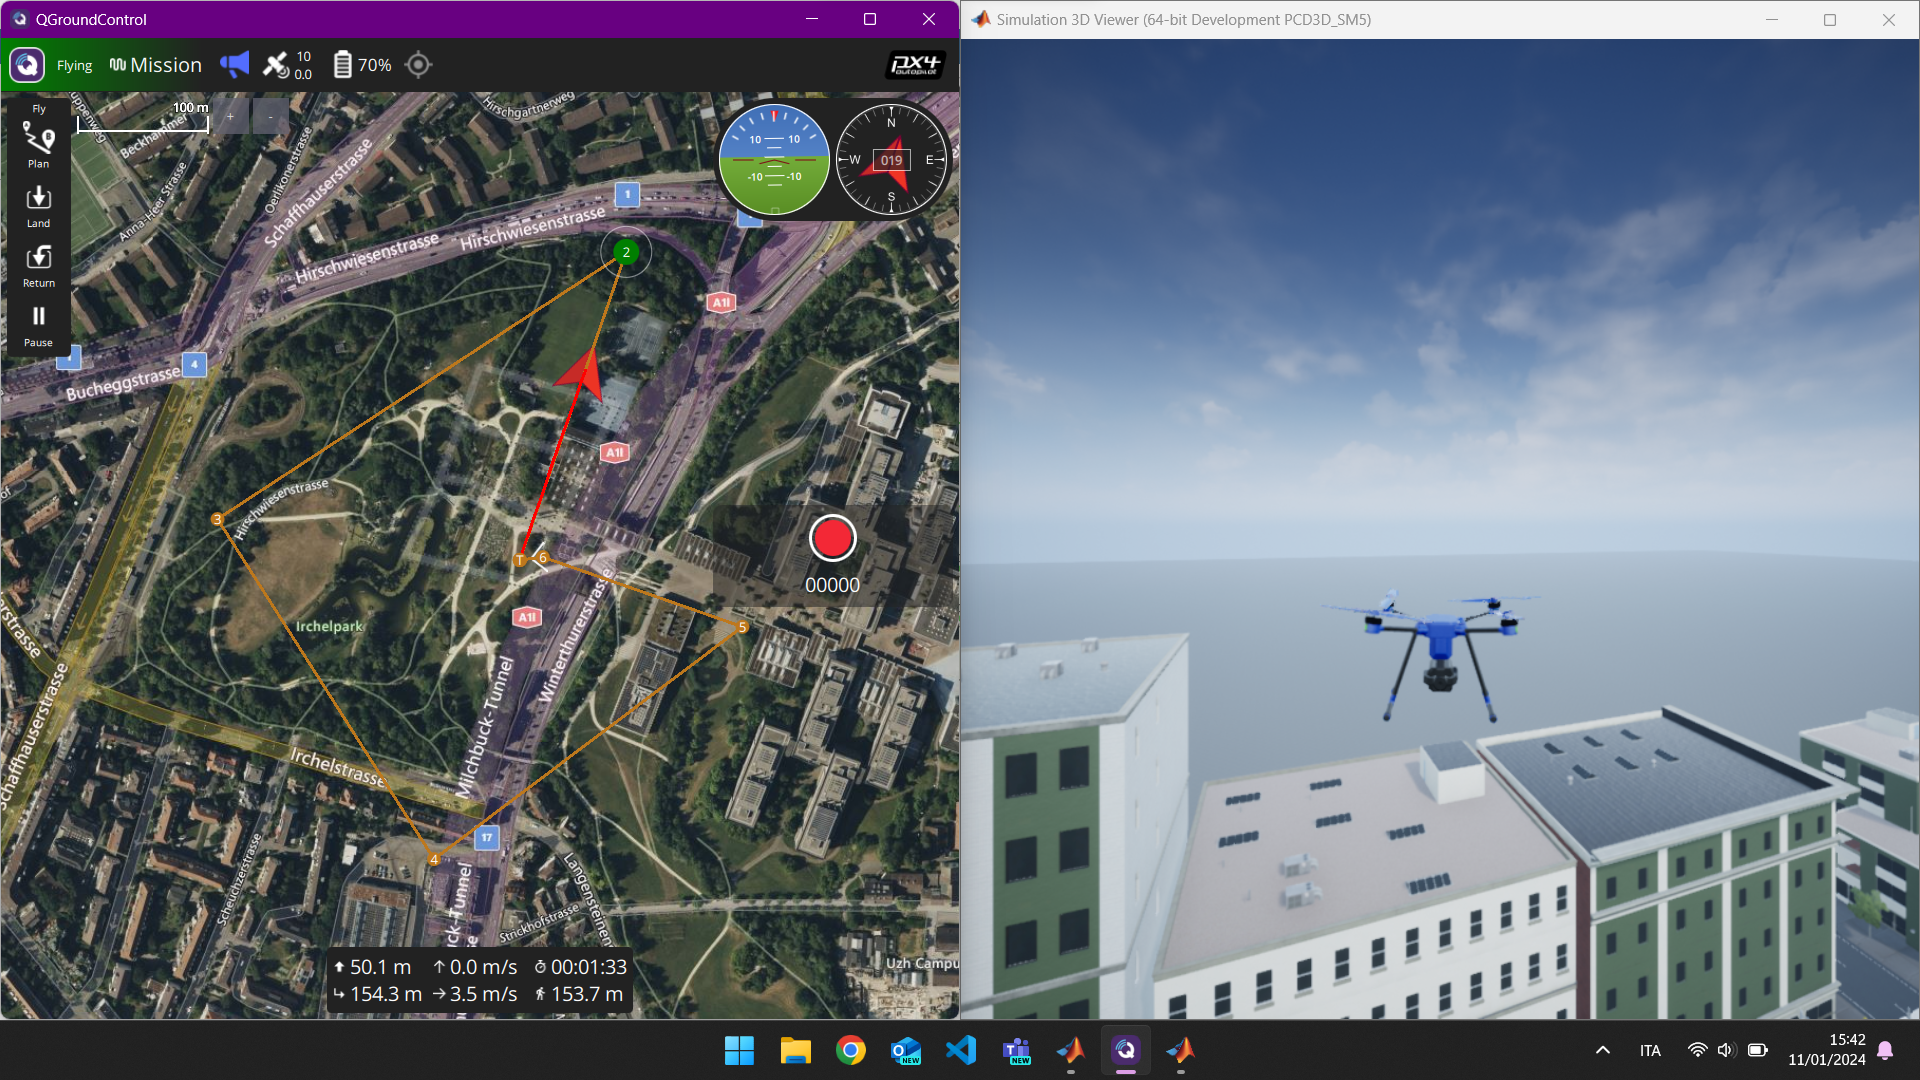
\includegraphics[width=\linewidth]{files/images/path1.png} % Imposta la larghezza dell'immagine al 50% della larghezza del testo
            \end{minipage}%
            \begin{minipage}[b]{0.5\linewidth} % Definisci la larghezza della seconda minipage (50% della larghezza della pagina)
                \centering
                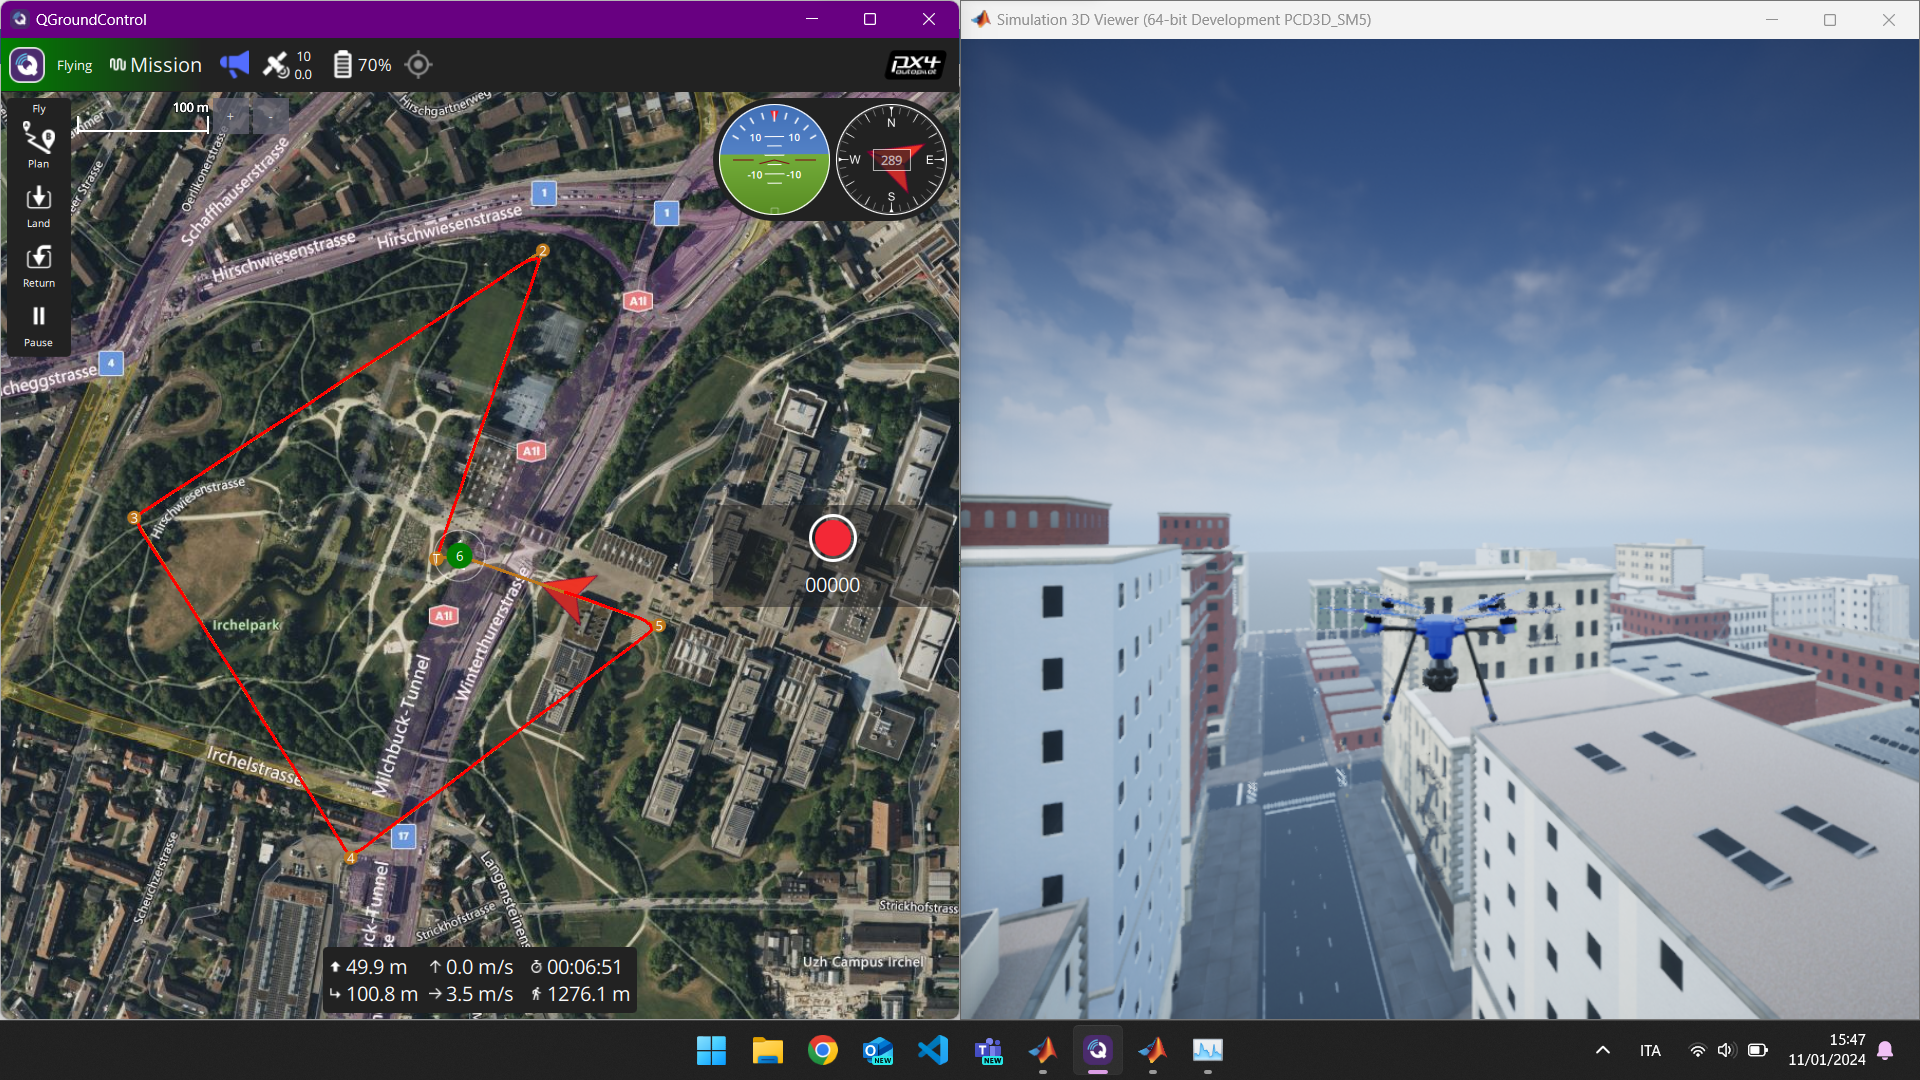
\includegraphics[width=\linewidth]{files/images/path1_finish.png} % Imposta la larghezza dell'immagine al 50% della larghezza del testo
            \end{minipage}
            \caption{Percorso di prova}
            \label{fig:Percorso di prova}
        \end{figure}
        
    \end{itemize}

    \item \textbf{Salvataggio e plot dati:}
    \begin{itemize}
        \item Dopo la conclusione della simulazione, uno script MATLAB preconfigurato viene eseguito per automatizzare il processo di visualizzazione e salvataggio dei dati in un file .mat.
        \item Questi dati includono informazioni vitali quali PWM motori, posizione (X, Y, Z), angoli di Eulero, velocità lineare, accelerazione lineare e velocità angolare.
        \item Lo script genera esegue il plot di ciascuna serie temporale. Questi grafici offrono una visione chiara e dettagliata delle dinamiche del drone durante la simulazione.
    \end{itemize}

    \item \textbf{Plot 3D del Percorso:}
    \begin{itemize}
        \item Utilizzando le informazioni sulla posizione (X, Y, Z) precedentemente registrate, un ulteriore script in MATLAB genera un plot tridimensionale del percorso seguito dal drone durante la simulazione. Questo plot consente di confrontare visivamente il percorso effettivamente percorso con quello inizialmente impostato (Fig. \ref{fig:Plot3D}).
        \begin{figure}[htbp]
            \begin{minipage}[b]{0.5\linewidth} % Definisci la larghezza della prima minipage (50% della larghezza della pagina)
              \centering
              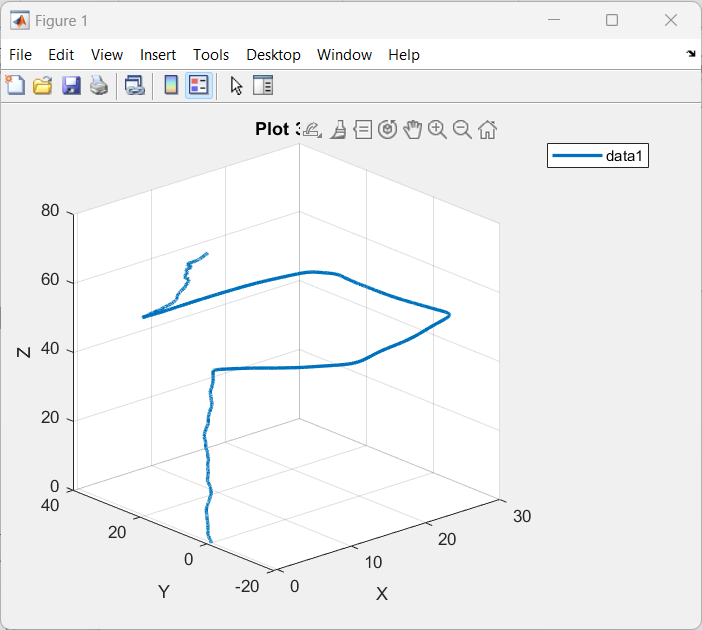
\includegraphics[width=\linewidth]{files/images/plot3D.png} % Imposta la larghezza dell'immagine al 50% della larghezza del testo
            \end{minipage}%
            \begin{minipage}[b]{0.5\linewidth} % Definisci la larghezza della seconda minipage (50% della larghezza della pagina)
                \centering
                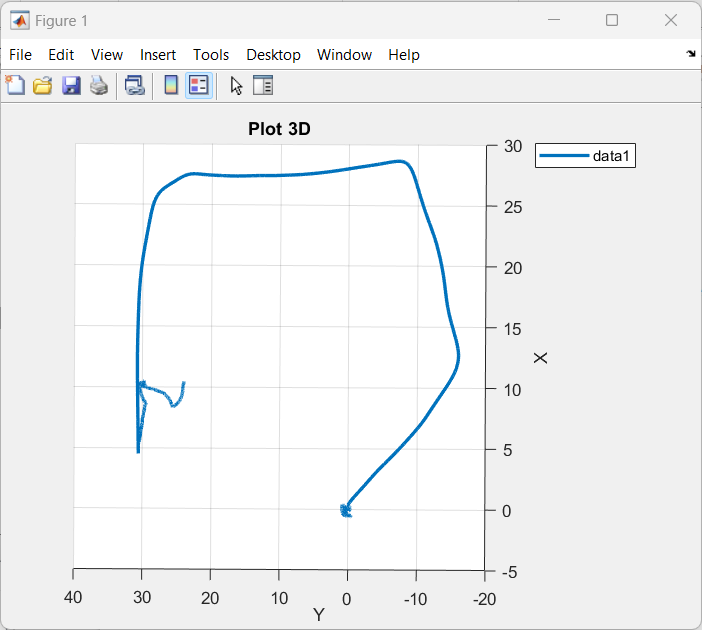
\includegraphics[width=\linewidth]{files/images/plot3D_1.png} % Imposta la larghezza dell'immagine al 50% della larghezza del testo
            \end{minipage}
            \caption{Plot 3D}
            \label{fig:Plot3D}
        \end{figure}
    \end{itemize}

    
\end{enumerate}








